
\documentclass{article}
\usepackage{amsmath}
\usepackage{graphicx}
\begin{document}

\section*{Topological Mass Fit for Leptons}

We hypothesize the mass of the $n$-th lepton is given by the topological formula:
\[
S(n) = A n^p - B n \log n \quad \text{with } p = 6.96
\]

\subsection*{Fit to Muon and Tau}

Using:
\begin{align*}
S(2) &= 105.658 \text{ MeV} \\
S(3) &= 1776.86 \text{ MeV}
\end{align*}

we solve for constants $A$ and $B$:

\[
A = 0.849014, \quad B = 0.031823
\]

\subsection*{Prediction for Electron (n = 1)}

Predicted mass:
\[
S(1) = 0.849014 \text{ MeV}
\]

Actual mass:
\[
m_e = 0.511 \text{ MeV}
\]

Difference:
\[
\Delta m = m_e - S(1) = -0.338014 \text{ MeV}
\]

This indicates a significant deviation for the electron, supporting the hypothesis that its mass arises from a different mechanism (e.g. electromagnetic self-energy), while the heavier generations follow the topological scaling.

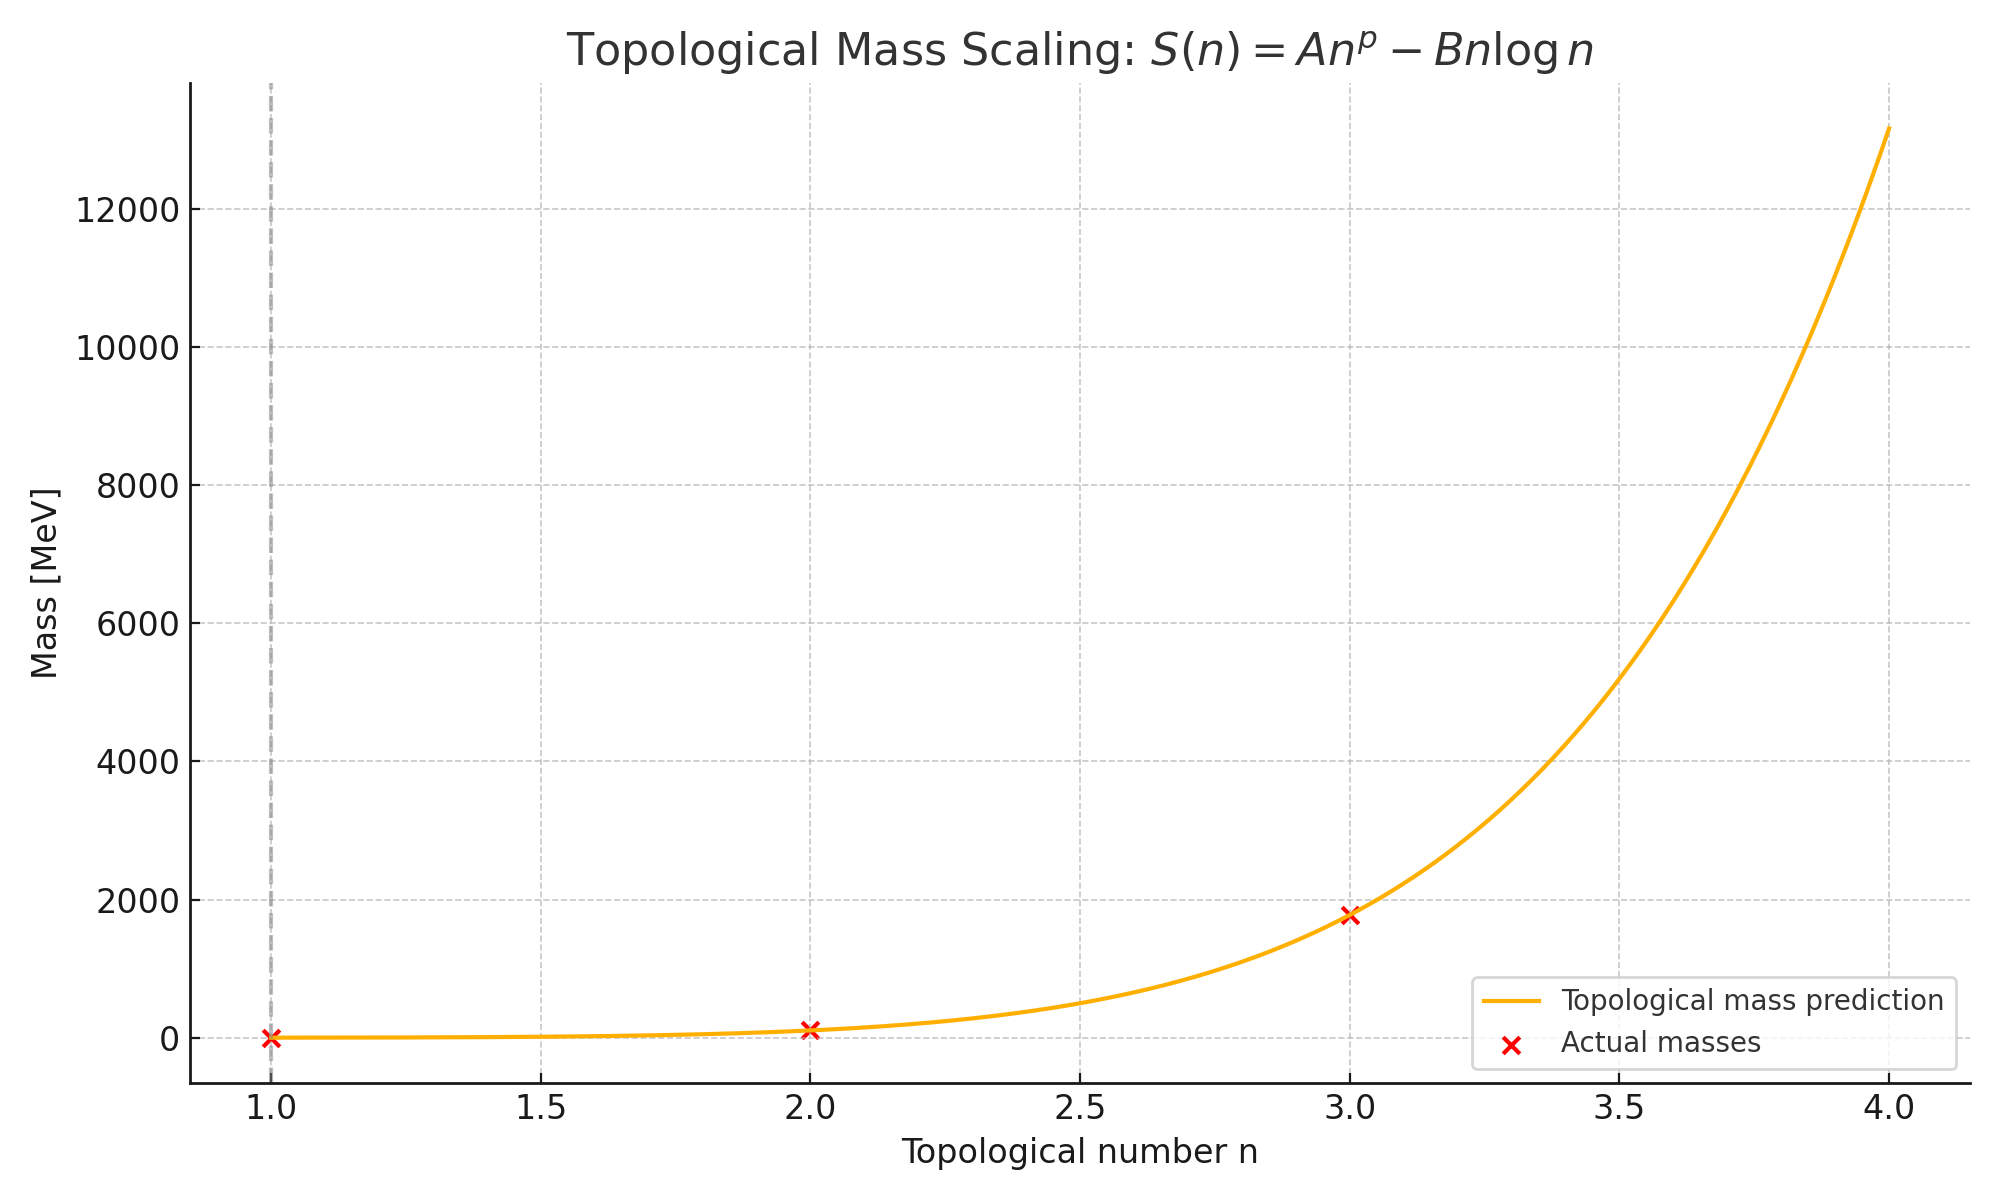
\includegraphics[width=\linewidth]{topological_mass_fit.png}

\end{document}
